%!TEX root = ../Thesis.tex
\chapter{Results}\label{cha:results}
%
\textcolor{red}{The results chapter should simply present the results of applying the methods presented in the method chapter without further ado. This chapter will typically contain many graphs, tables, etc. Sometimes it is natural to discuss the results as they are presented, combining them into a `Results and Discussion' chapter, but more often they are kept separate.}

This chapter will be used to look at the results from the objective and subjective measures and compare these against each other. There was a total of \textbf{NumOfParticipants} \todo{Add number of participants} participants which answered the subjective questionnaire. Figure \ref{fig:age} shows the age distribution of the participants, while figure \ref{fig:gender} shows the gender distribution. Table \textbf{TableNumber}\todo{Add correct reference once table is inserted} shows what type of occupation the participants had. 

For the statistical measures we plotted each of the questions to each video in histograms, along with error bars giving the standard deviation of the data set. The standard deviation was used to check the spread and variability of the data. We further looked at the histogram data manually to gather information from the result, but also checked for any statistical significant differences in the data. Since our data was not normally distributed, we went for a \textit{Mann-Whitney U test} \cite{wiki_mann-whitney}. From this we can use the p-value to decide on a statistical significance. 

\begin{figure}
\centering
\begin{minipage}{.5\textwidth}
  \centering
  \includegraphics[width=\linewidth]{img/Plots/pre/plot_age.png}
  \captionof{figure}{Age Distribution}
  \label{fig:age}
\end{minipage}%
\begin{minipage}{.5\textwidth}
  \centering
  \includegraphics[width=\linewidth]{img/Plots/pre/plot_gender.png}
  \captionof{figure}{Gender Distribution}
  \label{fig:gender}
\end{minipage}
\end{figure}

\todo{Insert table of occupations}

\section{Video 1}
\subsection{Objective Measures}

\begin{minipage}[c]{0.475\textwidth}
\begin{table}[H]
    \centering
    \begin{tabular}{||c c c||} 
        \hline
        \acrshort{iou} & \acrshort{dc} & \acrshort{pa} \\ [0.5ex] 
        \hline\hline
        93.590\% & 96.668\% & 99.220\% \\ [1ex] 
        \hline
    \end{tabular}
    \caption{Average metrics}
    \label{tab:metrics_video_1}
\end{table}
\end{minipage}
\begin{minipage}[c]{0.475\textwidth}
\begin{table}[H]
    \centering
    \begin{tabular}{||c c c||} 
        \hline
        \acrshort{tp} & \acrshort{tn} & \acrshort{fpn} \\ [0.5ex] 
        \hline\hline
        232890 & 1824538 & 16170 \\ [1ex] 
        \hline
    \end{tabular}
    \caption{Average pixel classification}
    \label{tab:pixels_video_1}
\end{table}
\end{minipage}

\subsection{Subjective Measures}

\begin{figure}[H]
    \centering
    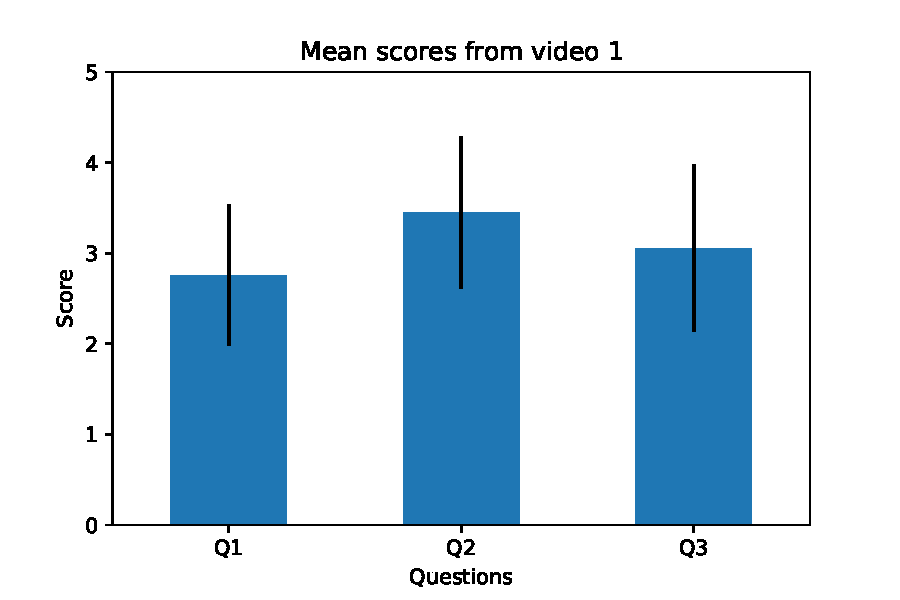
\includegraphics[width=0.6\textwidth]{img/subjective_measures/analysis/video_1.pdf}
    \caption{Subjective rating on video 1}
    \label{fig:visual_subj_vid1}
\end{figure}

\begin{table}[H]
    \centering
    \begin{tabular}{|c|c c c|} 
        \hline
           & \textbf{Mean Score} & \textbf{Percentage of full score} & \textbf{Standard Deviation} \\ [0.5ex] 
        \hline
        Q1 & 2.759 & 55.185\% & 0.775 \\ [1ex] 
        Q2 & 3.444 & 68.889\% & 0.839 \\ [1ex] 
        Q3 & 3.056 & 61.111\% & 0.920 \\ [1ex] 
        \hline
    \end{tabular}
    \caption{Numerical metrics from subjective rating in video 1}
    \label{tab:numerical_subj_vid1}
\end{table}

%------------------------------------

%------------------------------------

\section{Video 2}
\subsection{Objective Measures}

\begin{minipage}[c]{0.475\textwidth}
\begin{table}[H]
    \centering
    \begin{tabular}{||c c c||} 
        \hline
        \acrshort{iou} & \acrshort{dc} & \acrshort{pa} \\ [0.5ex] 
        \hline\hline
        94.097\% & 96.944\% & 99.281\% \\ [1ex] 
        \hline
    \end{tabular}
    \caption{Average metrics}
    \label{tab:metrics_video_2}
\end{table}
\end{minipage}
\begin{minipage}[c]{0.475\textwidth}
\begin{table}[H]
    \centering
    \begin{tabular}{||c c c||} 
        \hline
        \acrshort{tp} & \acrshort{tn} & \acrshort{fpn} \\ [0.5ex] 
        \hline\hline
        234287 & 1824412 & 14901 \\ [1ex] 
        \hline
    \end{tabular}
    \caption{Average pixel classification}
    \label{tab:pixels_video_11}
\end{table}
\end{minipage}

\subsection{Subjective Measures}

\begin{figure}[H]
    \centering
    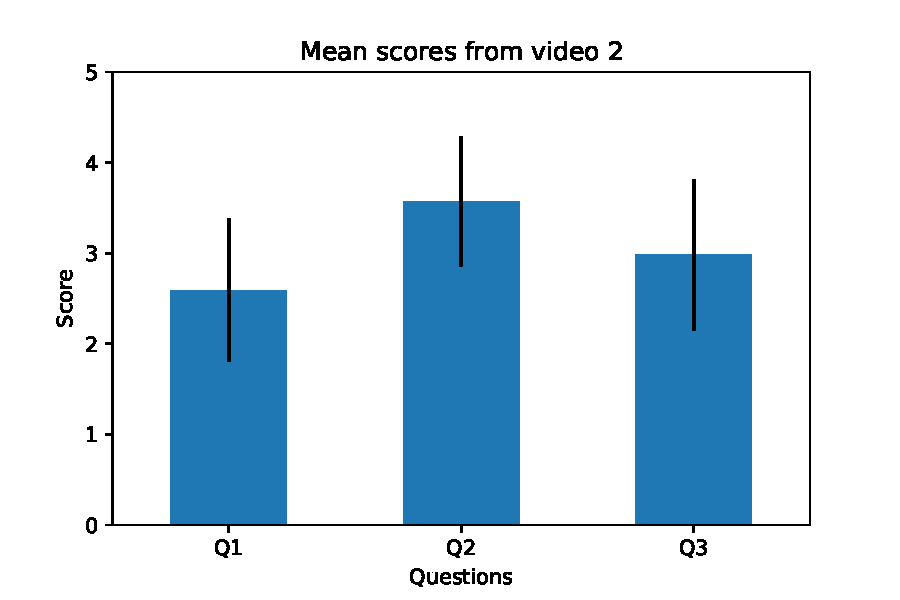
\includegraphics[width=0.6\textwidth]{img/subjective_measures/analysis/video_2.pdf}
    \caption{Subjective rating on video 2}
    \label{fig:visual_subj_vid2}
\end{figure}

\begin{table}[H]
    \centering
    \begin{tabular}{|c|c c c|} 
        \hline
           & \textbf{Mean Score} & \textbf{Percentage of full score} & \textbf{Standard Deviation} \\ [0.5ex] 
        \hline
        Q1 & 2.593 & 51.852\% & 0.790 \\ [1ex] 
        Q2 & 3.574 & 71.481\% & 0.716 \\ [1ex] 
        Q3 & 2.981 & 59.630\% & 0.835 \\ [1ex] 
        \hline
    \end{tabular}
    \caption{Numerical metrics from subjective rating in video 2}
    \label{tab:numerical_subj_vid2}
\end{table}

%------------------------------------

%------------------------------------

\section{Video 3}
\subsection{Objective Measures}

\begin{minipage}[c]{0.475\textwidth}
\begin{table}[H]
    \centering
    \begin{tabular}{||c c c||} 
        \hline
        \acrshort{iou} & \acrshort{dc} & \acrshort{pa} \\ [0.5ex] 
        \hline\hline
        95.096\% & 97.486\% & 99.406\% \\ [1ex] 
        \hline
    \end{tabular}
    \caption{Average metrics}
    \label{tab:metrics_video_3}
\end{table}
\end{minipage}
\begin{minipage}[c]{0.475\textwidth}
\begin{table}[H]
    \centering
    \begin{tabular}{||c c c||} 
        \hline
        \acrshort{tp} & \acrshort{tn} & \acrshort{fpn} \\ [0.5ex] 
        \hline\hline
        237919 & 1823370 & 12310 \\ [1ex] 
        \hline
    \end{tabular}
    \caption{Average pixel classification}
    \label{tab:pixels_video_3}
\end{table}
\end{minipage}

\subsection{Subjective Measures}

\begin{figure}[H]
    \centering
    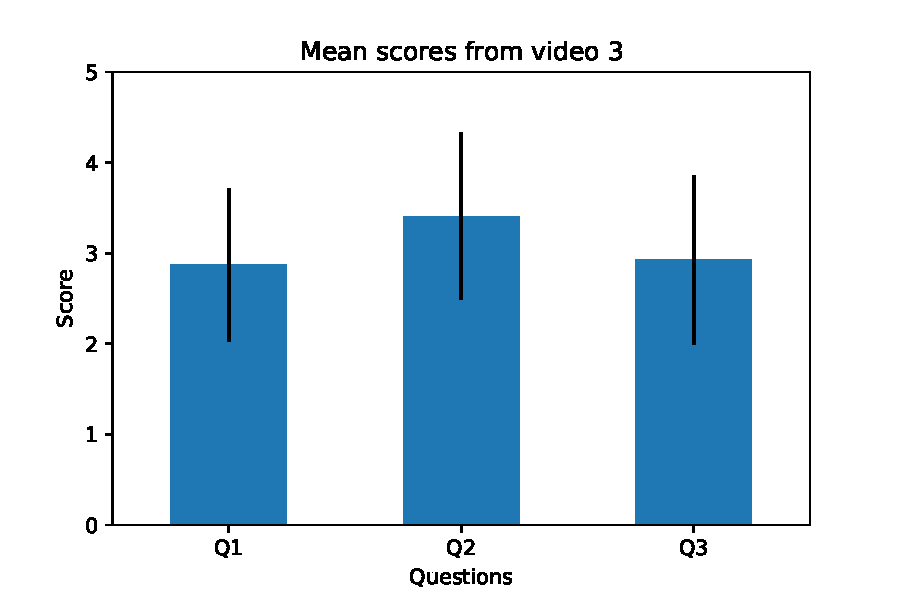
\includegraphics[width=0.6\textwidth]{img/subjective_measures/analysis/video_3.pdf}
    \caption{Subjective rating on video 3}
    \label{fig:visual_subj_vid3}
\end{figure}

\begin{table}[H]
    \centering
    \begin{tabular}{|c|c c c|} 
        \hline
           & \textbf{Mean Score} & \textbf{Percentage of full score} & \textbf{Standard Deviation} \\ [0.5ex] 
        \hline
        Q1 & 2.870 & 57.407\% & 0.848 \\ [1ex] 
        Q2 & 3.407 & 68.148\% & 0.922 \\ [1ex] 
        Q3 & 2.926 & 58.519\% & 0.929 \\ [1ex] 
        \hline
    \end{tabular}
    \caption{Numerical metrics from subjective rating in video 3}
    \label{tab:numerical_subj_vid3}
\end{table}



%------------------------------------

%------------------------------------

\section{Video 4}
\subsection{Objective Measures}

\begin{minipage}[c]{0.475\textwidth}
\begin{table}[H]
    \centering
    \begin{tabular}{||c c c||} 
        \hline
        \acrshort{iou} & \acrshort{dc} & \acrshort{pa} \\ [0.5ex] 
        \hline\hline
        94.719\% & 97.287\% & 99.354\% \\ [1ex] 
        \hline
    \end{tabular}
    \caption{Average metrics}
    \label{tab:metrics_video_4}
\end{table}
\end{minipage}
\begin{minipage}[c]{0.475\textwidth}
\begin{table}[H]
    \centering
    \begin{tabular}{||c c c||} 
        \hline
        \acrshort{tp} & \acrshort{tn} & \acrshort{fpn} \\ [0.5ex] 
        \hline\hline
        240444 & 1819753 & 13403 \\ [1ex] 
        \hline
    \end{tabular}
    \caption{Average pixel classification}
    \label{tab:pixels_video_4}
\end{table}
\end{minipage}

\subsection{Subjective Measures}

\begin{figure}[H]
    \centering
    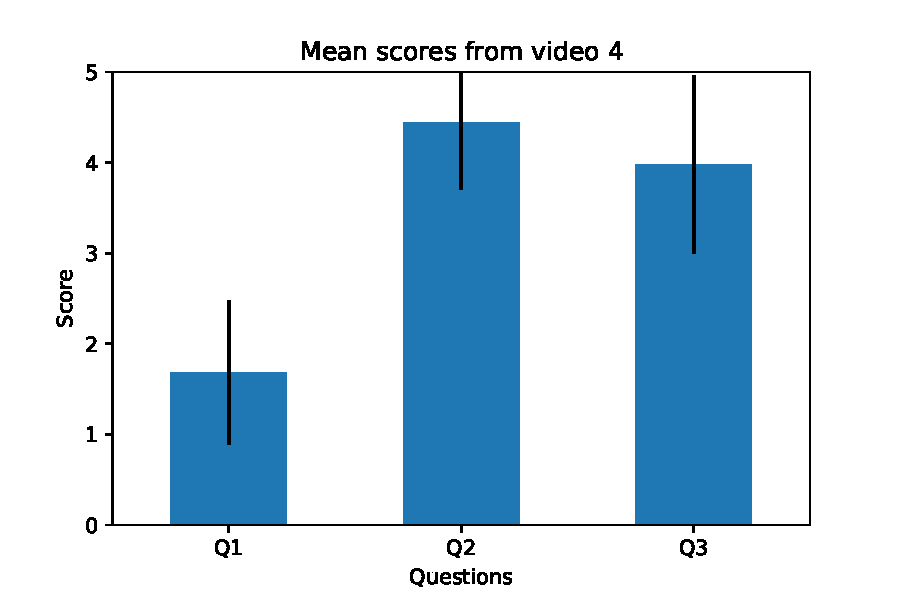
\includegraphics[width=0.6\textwidth]{img/subjective_measures/analysis/video_4.pdf}
    \caption{Subjective rating on video 4}
    \label{fig:visual_subj_vid4}
\end{figure}

\begin{table}[H]
    \centering
    \begin{tabular}{|c|c c c|} 
        \hline
           & \textbf{Mean Score} & \textbf{Percentage of full score} & \textbf{Standard Deviation} \\ [0.5ex] 
        \hline
        Q1 & 1.685 & 33.704\% & 0.797 \\ [1ex] 
        Q2 & 4.444 & 88.889\% & 0.744 \\ [1ex] 
        Q3 & 3.981 & 79.630\% & 0.981 \\ [1ex] 
        \hline
    \end{tabular}
    \caption{Numerical metrics from subjective rating in video 4}
    \label{tab:numerical_subj_vid4}
\end{table}


%------------------------------------

%------------------------------------

\section{Video 5}
\subsection{Objective Measures}

\begin{minipage}[c]{0.475\textwidth}
\begin{table}[H]
    \centering
    \begin{tabular}{||c c c||} 
        \hline
        \acrshort{iou} & \acrshort{dc} & \acrshort{pa} \\ [0.5ex] 
        \hline\hline
        94.812\% & 97.336\% & 99.366\% \\ [1ex] 
        \hline
    \end{tabular}
    \caption{Average metrics}
    \label{tab:metrics_video_5}
\end{table}
\end{minipage}
\begin{minipage}[c]{0.475\textwidth}
\begin{table}[H]
    \centering
    \begin{tabular}{||c c c||} 
        \hline
        \acrshort{tp} & \acrshort{tn} & \acrshort{fpn} \\ [0.5ex] 
        \hline\hline
        240427 & 1820023 & 13150 \\ [1ex] 
        \hline
    \end{tabular}
    \caption{Average pixel classification}
    \label{tab:pixels_video_5}
\end{table}
\end{minipage}

\subsection{Subjective Measures}

\begin{figure}[H]
    \centering
    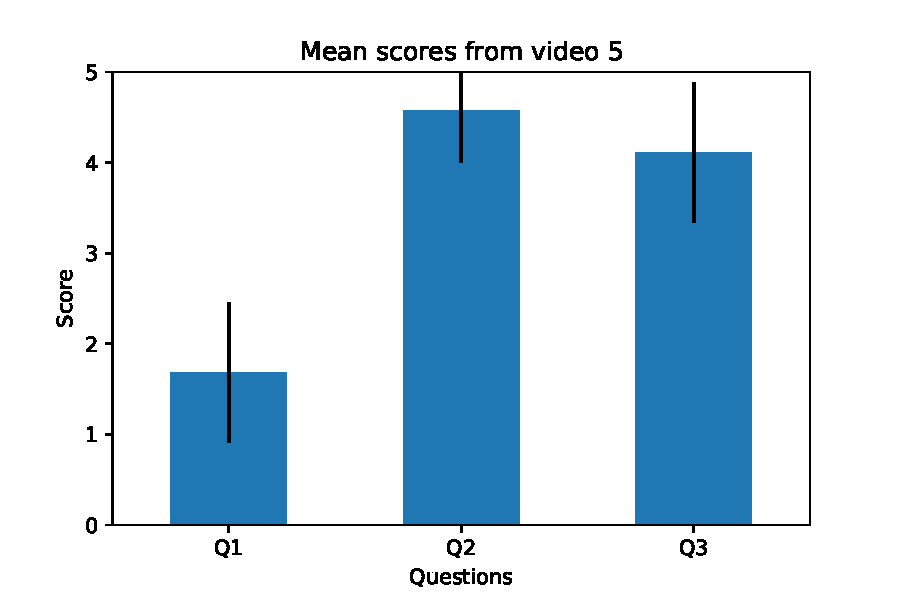
\includegraphics[width=0.6\textwidth]{img/subjective_measures/analysis/video_5.pdf}
    \caption{Subjective rating on video 5}
    \label{fig:visual_subj_vid5}
\end{figure}

\begin{table}[H]
    \centering
    \begin{tabular}{|c|c c c|} 
        \hline
           & \textbf{Mean Score} & \textbf{Percentage of full score} & \textbf{Standard Deviation} \\ [0.5ex] 
        \hline
        Q1 & 1.685 & 33.704\% & 0.773 \\ [1ex] 
        Q2 & 4.574 & 91.481\% & 0.570 \\ [1ex] 
        Q3 & 4.113 & 82.264\% & 0.776 \\ [1ex] 
        \hline
    \end{tabular}
    \caption{Numerical metrics from subjective rating in video 5}
    \label{tab:numerical_subj_vid5}
\end{table}


%------------------------------------

%------------------------------------
\section{Video 6}
\subsection{Objective Measures}

\begin{minipage}[c]{0.475\textwidth}
\begin{table}[H]
    \centering
    \begin{tabular}{||c c c||} 
        \hline
        \acrshort{iou} & \acrshort{dc} & \acrshort{pa} \\ [0.5ex] 
        \hline\hline
        94.239\% & 97.033\% & 99.292\% \\ [1ex] 
        \hline
    \end{tabular}
    \caption{Average metrics}
    \label{tab:metrics_video_6}
\end{table}
\end{minipage}
\begin{minipage}[c]{0.475\textwidth}
\begin{table}[H]
    \centering
    \begin{tabular}{||c c c||} 
        \hline
        \acrshort{tp} & \acrshort{tn} & \acrshort{fpn} \\ [0.5ex] 
        \hline\hline
        240430 & 1818482 & 14687 \\ [1ex] 
        \hline
    \end{tabular}
    \caption{Average pixel classification}
    \label{tab:pixels_video_6}
\end{table}
\end{minipage}

\subsection{Subjective Measures}

\begin{figure}[H]
    \centering
    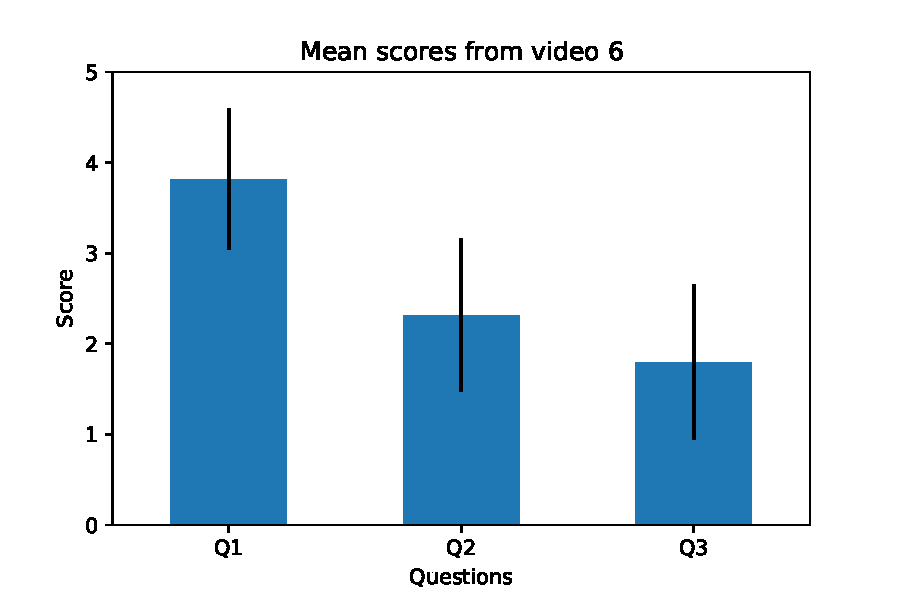
\includegraphics[width=0.6\textwidth]{img/subjective_measures/analysis/video_6.pdf}
    \caption{Subjective rating on video 6}
    \label{fig:visual_subj_vid6}
\end{figure}

\begin{table}[H]
    \centering
    \begin{tabular}{|c|c c c|} 
        \hline
           & \textbf{Mean Score} & \textbf{Percentage of full score} & \textbf{Standard Deviation} \\ [0.5ex] 
        \hline
        Q1 & 3.815 & 76.296\% & 0.779 \\ [1ex] 
        Q2 & 2.315 & 46.296\% & 0.843 \\ [1ex] 
        Q3 & 1.796 & 35.926\% & 0.855 \\ [1ex] 
        \hline
    \end{tabular}
    \caption{Numerical metrics from subjective rating in video 6}
    \label{tab:numerical_subj_vid6}
\end{table}

%------------------------------------

%------------------------------------

\section{Video 7}
\subsection{Objective Measures}

\begin{minipage}[c]{0.475\textwidth}
\begin{table}[H]
    \centering
    \begin{tabular}{||c c c||} 
        \hline
        \acrshort{iou} & \acrshort{dc} & \acrshort{pa} \\ [0.5ex] 
        \hline\hline
        93.909\% & 96.855\% & 99.216\% \\ [1ex] 
        \hline
    \end{tabular}
    \caption{Average metrics}
    \label{tab:metrics_video_7}
\end{table}
\end{minipage}
\begin{minipage}[c]{0.475\textwidth}
\begin{table}[H]
    \centering
    \begin{tabular}{||c c c||} 
        \hline
        \acrshort{tp} & \acrshort{tn} & \acrshort{fpn} \\ [0.5ex] 
        \hline\hline
        249856 & 1807490 & 16253 \\ [1ex] 
        \hline
    \end{tabular}
    \caption{Average pixel classification}
    \label{tab:pixels_video_7}
\end{table}
\end{minipage}

\subsection{Subjective Measures}

\begin{figure}[H]
    \centering
    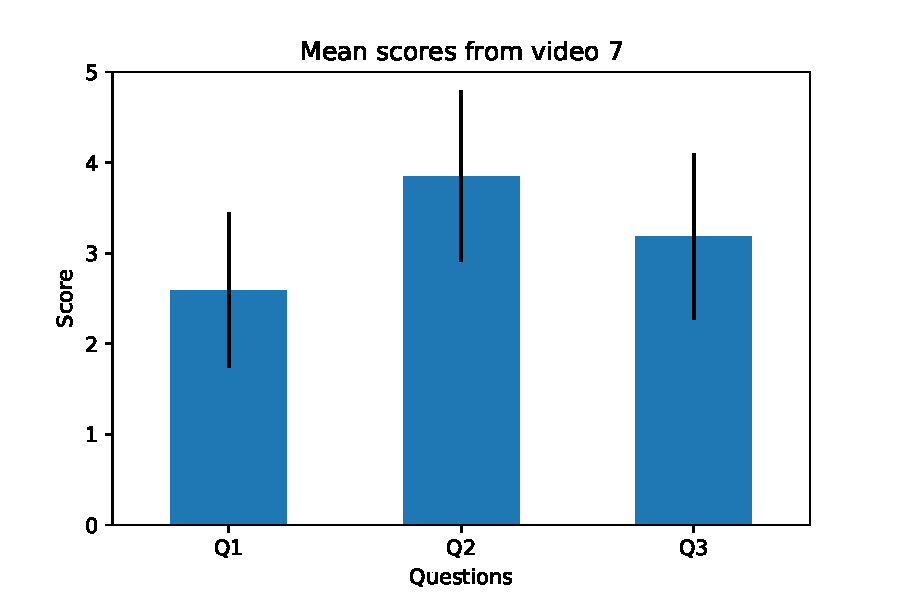
\includegraphics[width=0.6\textwidth]{img/subjective_measures/analysis/video_7.pdf}
    \caption{Subjective rating on video 7}
    \label{fig:visual_subj_vid7}
\end{figure}

\begin{table}[H]
    \centering
    \begin{tabular}{|c|c c c|} 
        \hline
           & \textbf{Mean Score} & \textbf{Percentage of full score} & \textbf{Standard Deviation} \\ [0.5ex] 
        \hline
        Q1 & 2.593 & 51.852\% & 0.858 \\ [1ex] 
        Q2 & 3.852 & 77.037\% & 0.940 \\ [1ex] 
        Q3 & 3.185 & 63.704\% & 0.913 \\ [1ex] 
        \hline
    \end{tabular}
    \caption{Numerical metrics from subjective rating in video 7}
    \label{tab:numerical_subj_vid7}
\end{table}

%------------------------------------

%------------------------------------

\section{Video 8}
\subsection{Objective Measures}

\begin{minipage}[c]{0.475\textwidth}
\begin{table}[H]
    \centering
    \begin{tabular}{||c c c||} 
        \hline
        \acrshort{iou} & \acrshort{dc} & \acrshort{pa} \\ [0.5ex] 
        \hline\hline
        94.749\% & 97.303\% & 99.332\% \\ [1ex] 
        \hline
    \end{tabular}
    \caption{Average metrics}
    \label{tab:metrics_video_8}
\end{table}
\end{minipage}
\begin{minipage}[c]{0.475\textwidth}
\begin{table}[H]
    \centering
    \begin{tabular}{||c c c||} 
        \hline
        \acrshort{tp} & \acrshort{tn} & \acrshort{fpn} \\ [0.5ex] 
        \hline\hline
        249735 & 1810021 & 13844 \\ [1ex] 
        \hline
    \end{tabular}
    \caption{Average pixel classification}
    \label{tab:pixels_video_8}
\end{table}
\end{minipage}

\subsection{Subjective Measures}

\begin{figure}[H]
    \centering
    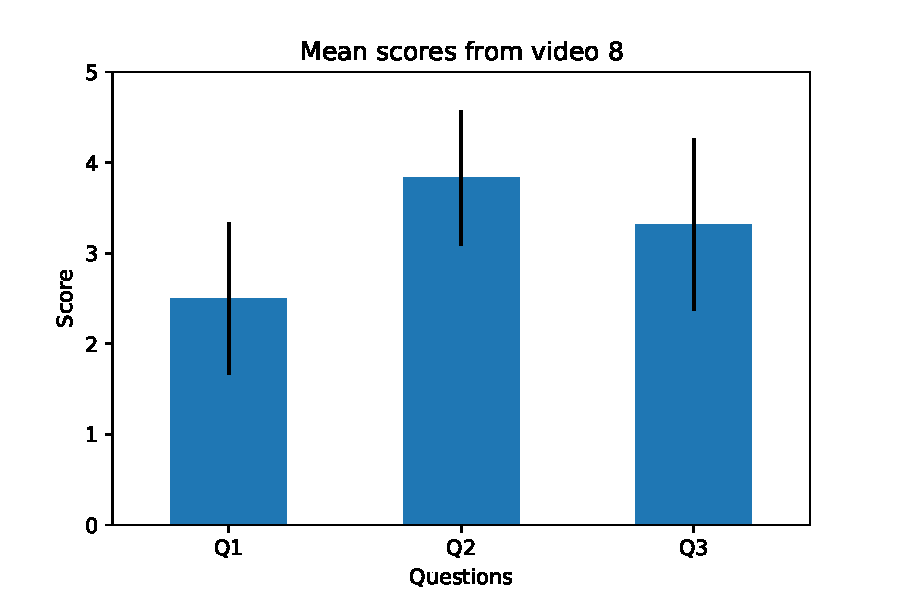
\includegraphics[width=0.6\textwidth]{img/subjective_measures/analysis/video_8.pdf}
    \caption{Subjective rating on video 8}
    \label{fig:visual_subj_vid8}
\end{figure}

\begin{table}[H]
    \centering
    \begin{tabular}{|c|c c c|} 
        \hline
           & \textbf{Mean Score} & \textbf{Percentage of full score} & \textbf{Standard Deviation} \\ [0.5ex] 
        \hline
        Q1 & 2.500 & 50.000\% & 0.841 \\ [1ex] 
        Q2 & 3.833 & 76.667\% & 0.746 \\ [1ex] 
        Q3 & 3.315 & 66.296\% & 0.948 \\ [1ex] 
        \hline
    \end{tabular}
    \caption{Numerical metrics from subjective rating in video 8}
    \label{tab:numerical_subj_vid8}
\end{table}

%------------------------------------

%------------------------------------

\section{Video 9}
\subsection{Objective Measures}

\begin{minipage}[c]{0.475\textwidth}
\begin{table}[H]
    \centering
    \begin{tabular}{||c c c||} 
        \hline
        \acrshort{iou} & \acrshort{dc} & \acrshort{pa} \\ [0.5ex] 
        \hline\hline
        93.687\% & 96.740\% & 99.187\% \\ [1ex] 
        \hline
    \end{tabular}
    \caption{Average metrics}
    \label{tab:metrics_video_9}
\end{table}
\end{minipage}
\begin{minipage}[c]{0.475\textwidth}
\begin{table}[H]
    \centering
    \begin{tabular}{||c c c||} 
        \hline
        \acrshort{tp} & \acrshort{tn} & \acrshort{fpn} \\ [0.5ex] 
        \hline\hline
        250392 & 1806340 & 16867 \\ [1ex] 
        \hline
    \end{tabular}
    \caption{Average pixel classification}
    \label{tab:pixels_video_9}
\end{table}
\end{minipage}

\subsection{Subjective Measures}

\begin{figure}[H]
    \centering
    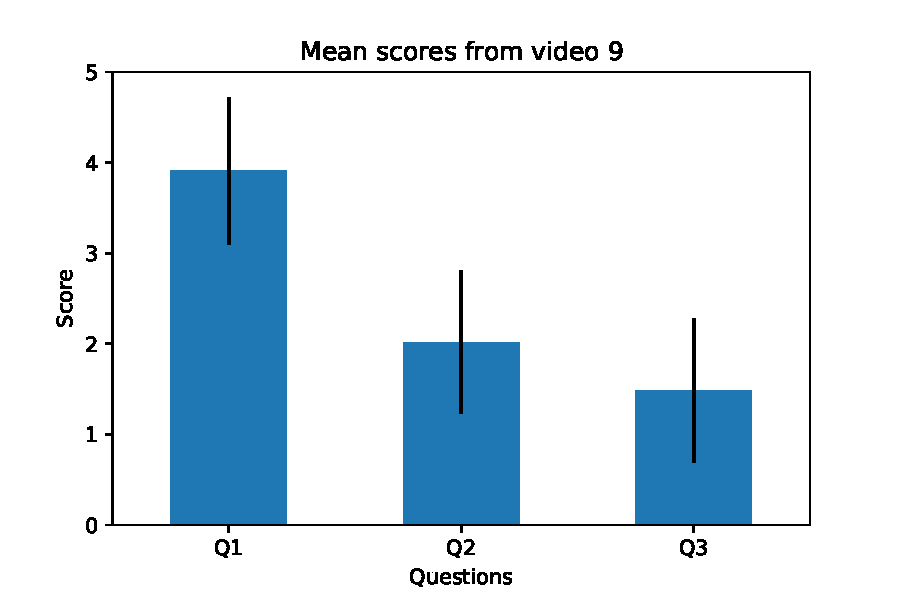
\includegraphics[width=0.6\textwidth]{img/subjective_measures/analysis/video_9.pdf}
    \caption{Subjective rating on video 9}
    \label{fig:visual_subj_vid9}
\end{figure}

\begin{table}[H]
    \centering
    \begin{tabular}{|c|c c c|} 
        \hline
           & \textbf{Mean Score} & \textbf{Percentage of full score} & \textbf{Standard Deviation} \\ [0.5ex] 
        \hline
        Q1 & 3.907 & 78.148\% & 0.807 \\ [1ex] 
        Q2 & 2.019 & 40.370\% & 0.789 \\ [1ex] 
        Q3 & 1.481 & 29.630\% & 0.795 \\ [1ex] 
        \hline
    \end{tabular}
    \caption{Numerical metrics from subjective rating in video 9}
    \label{tab:numerical_subj_vid9}
\end{table}

%------------------------------------

%------------------------------------


\section{Video 10}
\subsection{Objective Measures}

\begin{minipage}[c]{0.475\textwidth}
\begin{table}[H]
    \centering
    \begin{tabular}{||c c c||} 
        \hline
        \acrshort{iou} & \acrshort{dc} & \acrshort{pa} \\ [0.5ex] 
        \hline\hline
        93.982\% & 96.897\% & 99.240\% \\ [1ex] 
        \hline
    \end{tabular}
    \caption{Average metrics}
    \label{tab:metrics_video_10}
\end{table}
\end{minipage}
\begin{minipage}[c]{0.475\textwidth}
\begin{table}[H]
    \centering
    \begin{tabular}{||c c c||} 
        \hline
        \acrshort{tp} & \acrshort{tn} & \acrshort{fpn} \\ [0.5ex] 
        \hline\hline
        245813 & 1812035 & 15751 \\ [1ex] 
        \hline
    \end{tabular}
    \caption{Average pixel classification}
    \label{tab:pixels_video_10}
\end{table}
\end{minipage}

\subsection{Subjective Measures}

\begin{figure}[H]
    \centering
    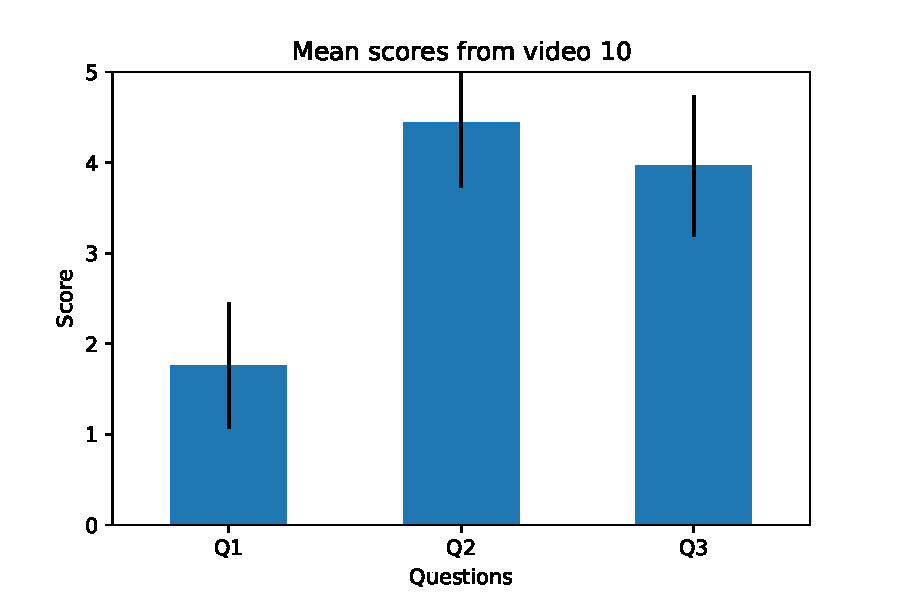
\includegraphics[width=0.6\textwidth]{img/subjective_measures/analysis/video_10.pdf}
    \caption{Subjective rating on video 10}
    \label{fig:visual_subj_vid10}
\end{figure}

\begin{table}[H]
    \centering
    \begin{tabular}{|c|c c c|} 
        \hline
           & \textbf{Mean Score} & \textbf{Percentage of full score} & \textbf{Standard Deviation} \\ [0.5ex] 
        \hline
        Q1 & 1.759 & 35.185\% & 0.699 \\ [1ex] 
        Q2 & 4.444 & 88.889\% & 0.718 \\ [1ex] 
        Q3 & 3.963 & 79.259\% & 0.776 \\ [1ex] 
        \hline
    \end{tabular}
    \caption{Numerical metrics from subjective rating in video 10}
    \label{tab:numerical_subj_vid10}
\end{table}

%------------------------------------

%------------------------------------

\section{Video 11}
\subsection{Objective Measures}

\begin{minipage}[c]{0.475\textwidth}
\begin{table}[H]
    \centering
    \begin{tabular}{||c c c||} 
        \hline
        \acrshort{iou} & \acrshort{dc} & \acrshort{pa} \\ [0.5ex] 
        \hline\hline
        94.166\% & 96.995\% & 99.265\% \\ [1ex] 
        \hline
    \end{tabular}
    \caption{Average metrics}
    \label{tab:metrics_video_11}
\end{table}
\end{minipage}
\begin{minipage}[c]{0.475\textwidth}
\begin{table}[H]
    \centering
    \begin{tabular}{||c c c||} 
        \hline
        \acrshort{tp} & \acrshort{tn} & \acrshort{fpn} \\ [0.5ex] 
        \hline\hline
        245737 & 1812624 & 15239 \\ [1ex] 
        \hline
    \end{tabular}
    \caption{Average pixel classification}
    \label{tab:pixels_video_11}
\end{table}
\end{minipage}

\subsection{Subjective Measures}

\begin{figure}[H]
    \centering
    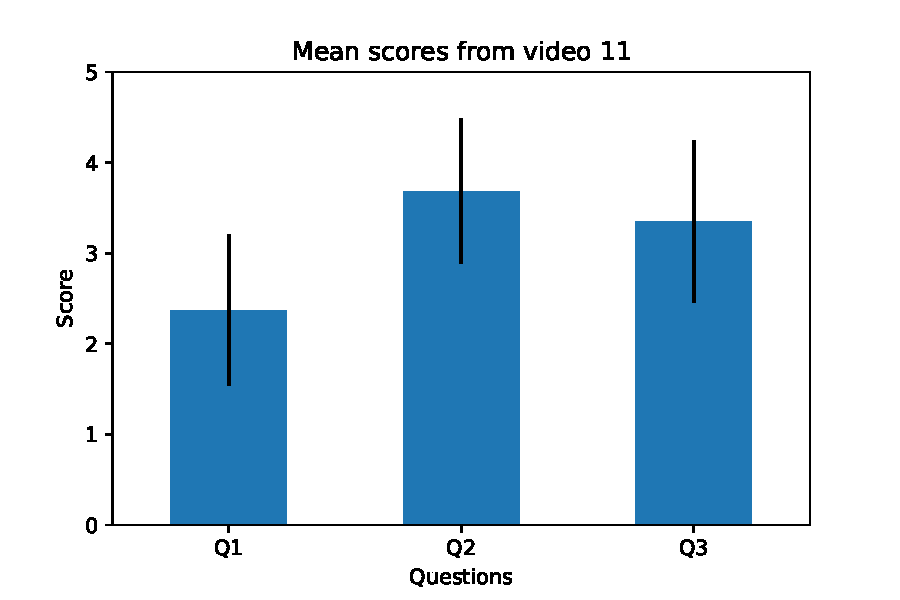
\includegraphics[width=0.6\textwidth]{img/subjective_measures/analysis/video_11.pdf}
    \caption{Subjective rating on video 11}
    \label{fig:visual_subj_vid11}
\end{figure}

\begin{table}[H]
    \centering
    \begin{tabular}{|c|c c c|} 
        \hline
           & \textbf{Mean Score} & \textbf{Percentage of full score} & \textbf{Standard Deviation} \\ [0.5ex] 
        \hline
        Q1 & 2.370 & 47.407\% & 0.831 \\ [1ex] 
        Q2 & 3.685 & 73.704\% & 0.797 \\ [1ex] 
        Q3 & 3.352 & 67.037\% & 0.894 \\ [1ex] 
        \hline
    \end{tabular}
    \caption{Numerical metrics from subjective rating in video 11}
    \label{tab:numerical_subj_vid11}
\end{table}


%------------------------------------

%------------------------------------

\section{Video 12}
\subsection{Objective Measures}

\begin{minipage}[c]{0.475\textwidth}
\begin{table}[H]
    \centering
    \begin{tabular}{||c c c||} 
        \hline
        \acrshort{iou} & \acrshort{dc} & \acrshort{pa} \\ [0.5ex] 
        \hline\hline
        93.845\% & 96.834\% & 99.220\% \\ [1ex] 
        \hline
    \end{tabular}
    \caption{Average metrics}
    \label{tab:metrics_video_12}
\end{table}
\end{minipage}
\begin{minipage}[c]{0.475\textwidth}
\begin{table}[H]
    \centering
    \begin{tabular}{||c c c||} 
        \hline
        \acrshort{tp} & \acrshort{tn} & \acrshort{fpn} \\ [0.5ex] 
        \hline\hline
        246300 & 181136 & 16164 \\ [1ex] 
        \hline
    \end{tabular}
    \caption{Average pixel classification}
    \label{tab:pixels_video_12}
\end{table}
\end{minipage}

\subsection{Subjective Measures}

\begin{figure}[H]
    \centering
    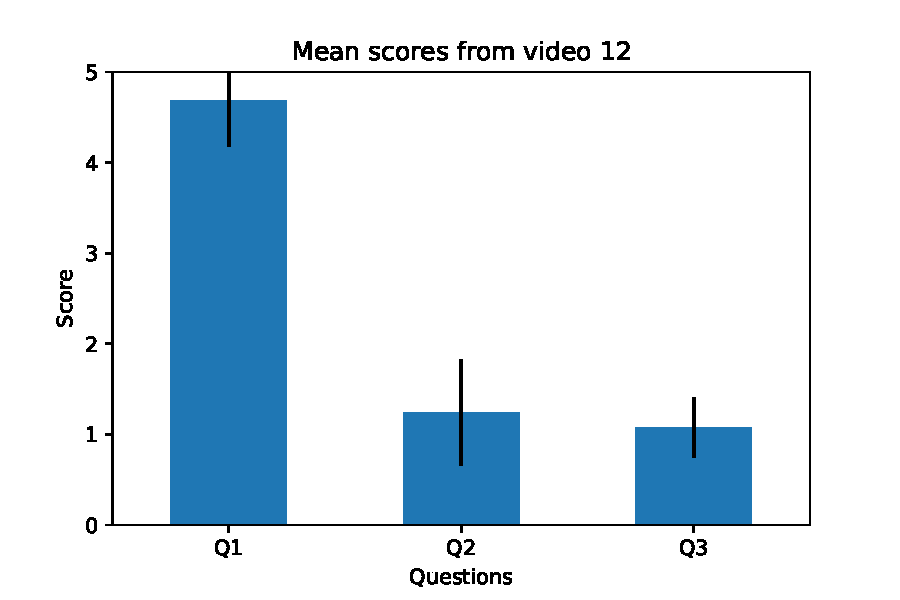
\includegraphics[width=0.6\textwidth]{img/subjective_measures/analysis/video_12.pdf}
    \caption{Subjective rating on video 12}
    \label{fig:visual_subj_vid12}
\end{figure}

\begin{table}[H]
    \centering
    \begin{tabular}{|c|c c c|} 
        \hline
           & \textbf{Mean Score} & \textbf{Percentage of full score} & \textbf{Standard Deviation} \\ [0.5ex] 
        \hline
        Q1 & 4.685 & 93.704\% & 0.507 \\ [1ex] 
        Q2 & 1.241 & 24.815\% & 0.581 \\ [1ex] 
        Q3 & 1.074 & 21.481\% & 0.328 \\ [1ex] 
        \hline
    \end{tabular}
    \caption{Numerical metrics from subjective rating in video 12}
    \label{tab:numerical_subj_vid12}
\end{table}


\subsection{Qualitative Feedback}
The participants were able to provide some additional feedback at the end of the questionnaire if they wanted to. The comments were as follows:
\begin{table}[H]
    \centering
    \begin{tabular}{p{12cm}} 
        \hline
        \lipsum[2] \\
        \hline
        \lipsum[2] \\
        \hline
    \end{tabular}
    \caption{Qualitative feedback from participants}
    \label{tab:comments}
\end{table}
\todo{Fill in comments}